\documentclass{article}
\usepackage{CJKutf8, indentfirst, graphicx, subfigure}
\begin{document}
\begin{CJK}{UTF8}{bsmi}
\title{硬體設計與實驗 Lab6 Report}
\author{104021219 鄭余玄}
\date{}
\maketitle
\section{實做過程}
lab\_6 主程式是沿用 lab\_5 的程式碼,除了增加一元的輸入輸出訊號,另外就是把訊號輸入來源改成鍵盤。
此外,因為輸入訊號來源是鍵盤,所以只有cancel 訊號需要 debounce 和產生 onepulse。
鍵盤輸入訊號處理的部份,我是分開在 Keyboard\_Signal 這個模組中處理。

Keyboard\_Signal 主要是參考助教的 SimpleDisplay,但是這次鍵盤主要只會按下一個鍵,頂多同時按 shift,所以 last\_change 訊號沒有用到。
此外,KEY\_CODES 陣列可以直接用 9'h 去寫十六進位的數值,就不用特地去轉成二進位。
而 KeyboardDecoder 的輸入訊號,需要先經過 LargePulse 處理,把一個訊號延長 $2^{16}$ 倍。
LargePulse 的實做方法也是參考助教提供的 FSM,用兩個狀態加上 up counter 就可以完成實做了。

\subsection{Block diagram}
\begin{figure*}[h]
\centering{
  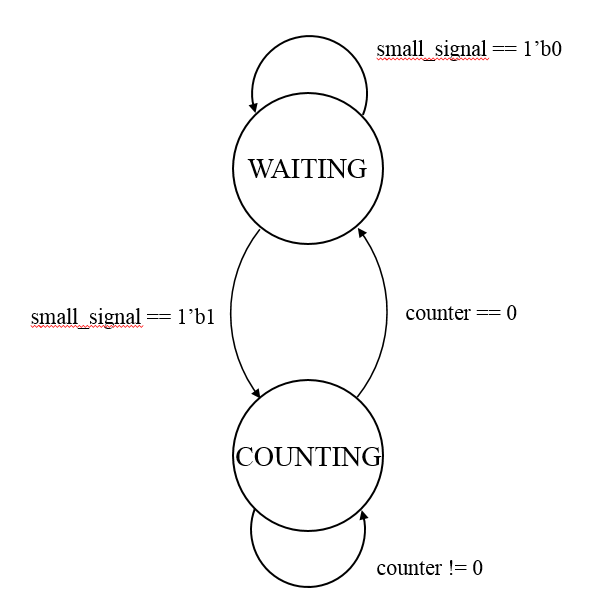
\includegraphics[width=.5\textwidth, angle=0]{LargePulse}
}
\caption{Block diagrams: LargePulse.}
\end{figure*}

\section{學到的東西及遇到的困難}
這次學到的東西就是 PS/2 訊號的處理和原理,還有 IP 的使用。
上次老師上課對於 IP 好像很有疑問,不過我覺得助教會使用 IP 是因為,那些電路已經是合成實做好的。
如果只是加入 .v 檔案,那可能會因為不同編譯環境而產生不同的電路,這樣可能就不會產生最佳的電路。

\section{想對老師或助教說的話}
覺得助教可以對 lab 內容多做一些說明,像是 LongPulse 講解就很趕,因此對於功能和用法都需要自己再多想一下。

\end{CJK}
\end{document}
